%%%%%%%%%%%%%%%%%%%%%%%%%%%%%%%%%%%%%%%%%
% Beamer Presentation
% LaTeX Template
% Version 1.0 (10/11/12)
%
% This template has been downloaded from:
% http://www.LaTeXTemplates.com
%
% License:
% CC BY-NC-SA 3.0 (http://creativecommons.org/licenses/by-nc-sa/3.0/)
%
%%%%%%%%%%%%%%%%%%%%%%%%%%%%%%%%%%%%%%%%%

%----------------------------------------------------------------------------------------
%	PACKAGES AND THEMES
%----------------------------------------------------------------------------------------

\documentclass{beamer}
\usepackage[utf8]{inputenc}
\usepackage{pifont}
\usepackage{svg}
\newcommand{\cmark}{\ding{51}}%
\newcommand{\xmark}{\ding{55}}%
\newcommand{\done}{\rlap{$\square$}{\raisebox{2pt}{\large\hspace{1pt}\cmark}}%
\hspace{-2.5pt}}
\newcommand{\wontfix}{\rlap{$\square$}{\large\hspace{1pt}\xmark}}
\addtobeamertemplate{navigation symbols}{}{%
    \usebeamerfont{footline}%
    \usebeamercolor[fg]{footline}%
    \hspace{1em}%
    \insertframenumber/\inserttotalframenumber
}

\mode<presentation> {

% The Beamer class comes with a number of default slide themes
% which change the colors and layouts of slides. Below this is a list
% of all the themes, uncomment each in turn to see what they look like.

%\usetheme{default}
%\usetheme{AnnArbor}
%\usetheme{Antibes}
%\usetheme{Bergen}
%\usetheme{Berkeley}
%\usetheme{Berlin}
%\usetheme{Boadilla}
%\usetheme{CambridgeUS}
%\usetheme{Copenhagen}
%\usetheme{Darmstadt}
%\usetheme{Dresden}
%\usetheme{Frankfurt}
%\usetheme{Goettingen}
\usetheme{Hannover}
%\usetheme{Ilmenau}
%\usetheme{JuanLesPins}
%\usetheme{Luebeck}
%\usetheme{Madrid}
%\usetheme{Malmoe}
%\usetheme{Marburg}
%\usetheme{Montpellier}%
%\usetheme{PaloAlto}
%\usetheme{Pittsburgh}
%\usetheme{Rochester}
%\usetheme{Singapore}
%\usetheme{Szeged}
%\usetheme{Warsaw}

% As well as themes, the Beamer class has a number of color themes
% for any slide theme. Uncomment each of these in turn to see how it
% changes the colors of your current slide theme.

%\usecolortheme{albatross}
%\usecolortheme{beaver}
%\usecolortheme{beetle}
%\usecolortheme{crane}
\usecolortheme{dolphin}
%\usecolortheme{dove}
%\usecolortheme{fly}
%\usecolortheme{lily}
%\usecolortheme{orchid}
%\usecolortheme{rose}
%\usecolortheme{seagull}
%\usecolortheme{seahorse}
%\usecolortheme{whale}
%\usecolortheme{wolverine}

%\setbeamertemplate{footline} % To remove the footer line in all slides uncomment this line
%\setbeamertemplate{footline}[page number] % To replace the footer line in all slides with a simple slide count uncomment this line

%\setbeamertemplate{navigation symbols}{} % To remove the navigation symbols from the bottom of all slides uncomment this line
}

\usepackage{graphicx} % Allows including images
\usepackage{booktabs} % Allows the use of \toprule, \midrule and \bottomrule in tables
\usepackage{amsmath}
\usepackage{skmath}
\usepackage{csquotes}
\usepackage{datetime}
\usepackage{breakcites}


\ExplSyntaxOn
\RenewDocumentCommand\log{oom}{%
  \IfNoValueTF{#1}
    {\ensuremath{\__skmath_log:\IfNoValueTF{#2}{}{\c_math_superscript_token{#2}}\__skmath_parens:n{#3}}}
    {\ensuremath{\__skmath_log:\c_math_subscript_token{#1}\IfNoValueTF{#2}{}{\c_math_superscript_token{#2}}\__skmath_parens:n{#3}}}%
}
\ExplSyntaxOff

\setbeamertemplate{itemize items}[default]

%----------------------------------------------------------------------------------------
%	TITLE PAGE
%----------------------------------------------------------------------------------------
\title[Text Entailment Seminar] %optional
{An ontology-based approach to model qualitative world knowledge extracted from product reviews for use in QA systems}
\author[]{\Large Thomas Huber\texorpdfstring{\\ \small \vspace{1cm} \color{black}}{ }}
\date[\today] % (optional)
{\today}
\begin{document}
\frame{\titlepage}

\section{Introduction}
\begin{frame}
\frametitle{General idea}
\begin{itemize}
    \item For a category of products find out which specific features each \textbf{individual} product has and how good the feature is \textit{for that specific product}
	\item Store the information in an RDF ontology
    \item Use the stored information to answer queries about specific products such as: \textit{Which drills are best for wood?}
\end{itemize}
\end{frame}

\section{Plan}
\subsection{Scraping}
\begin{frame}{Scraping}
    \begin{itemize}
        \item The reviews needed will be scraped by me from Amazon.com
        \item The product category will be \textit{drills}
        \item Technical products / machines have a lot of features and generally a lot of reviews
        \item I am aiming for a few hundred specific products to get nice results, but the system would work with less or more reviews
    \end{itemize}
\end{frame}

\subsection{Feature extraction}
\begin{frame}{Feature extraction}
\begin{itemize}
    \item Based on the system "Red Opal"\\
        \cite{scaffidi2007red}
    \item The general idea is to extract nouns from reviews that occur more often in the reviews than they do normally (the features a product has) and assign a score based on the rating
    \item To find unnaturally often occurring nouns, a frequency list is used
    \item I will use word frequencies from Wikipedia, as provided by the University of Leipzig \url{http://wortschatz.uni-leipzig.de/de/download}
\end{itemize}
\end{frame}

\subsection{Ontology building}
\begin{frame}{Ontology building}
\begin{itemize}
    \item The extracted information (which specific product has which feature and the score for that feature) will be modeled in RDF
    \item :someDrill :hasFeature :someFeature .
    \item :someFeature :hasLabel "charger" .
    \item :someFeature :hasScore 3.0\^\^xsd:double .
    \item The model will be extended with WordNet definitions
\end{itemize}
\end{frame}

\begin{frame}{Ontology building - Example}
    \begin{figure}[htbp]
      \centering
      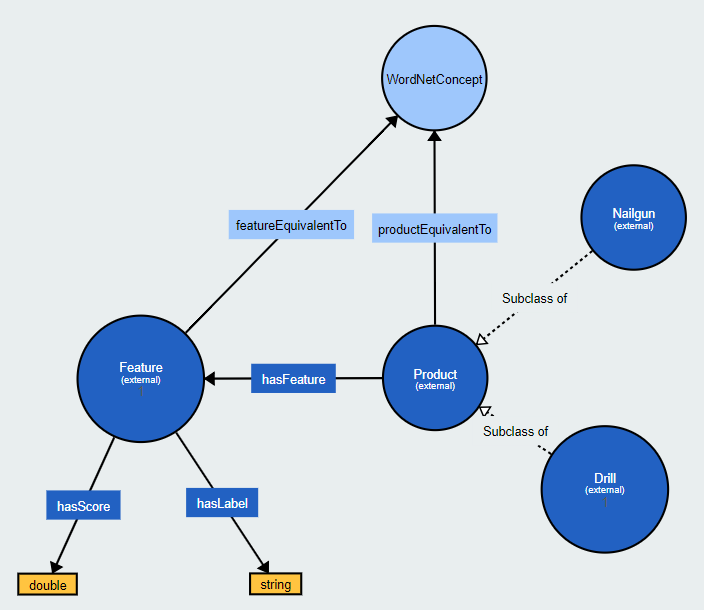
\includegraphics[scale=0.5]{textentailment.PNG}
    \end{figure}
\end{frame}

\section{The role of text entailment}
\begin{frame}{The role of text entailment}
    \begin{itemize}
        \item \textbf{Which drills make the cleanest holes?}
        \item \textit{make\_holes} is the action
        \item \textit{drill} is the category of products
        \item use a graph similar to the WordNetGraph described in "Recognizing and Justifying Text Entailment through Distributional Navigation on Definition Graphs" \cite{silva2018recognizing} to find everything that can make holes or be used to make them
        \item search a path between the extracted features and \textit{make\_holes} and then check which specific products have a high score for features that have a path
    \end{itemize}
\end{frame}

\section{Related work}
\begin{frame}{Related work I}
\begin{itemize}
    \item "Effective Collaboration in Product Development via a Common Sharable Ontology"\\ \cite{mostefai2005effective}\\
    An ontology over individual parts of a product as part of product development. Could by extended by my data to find out which individual parts belong to features the users do not like to replace or improve them.
\end{itemize}
\end{frame}

\begin{frame}{Related work II}
    \begin{itemize}
        \item Informed Recommender: Basing Recommendations on Consumer Product Reviews \cite{aciar2007informed}
        \item This system processes reviews of individual products and uses sentiment analysis and machine learning to find out which features the users like and dislike
        \item Uses the extracted information to recommend products, but does not make use of text entailment to answer queries
        \item The features have to be defined by hand and for each category training their classifier is required
        \item However it takes into account the skill level of the reviewer to adjust the score
        \item As future work, the skill level consideration part of this system could be incorporated into my system to adjust the scoring
    \end{itemize}
\end{frame}

\begin{frame}{Related work II}
    \begin{figure}[htbp]
      \centering
      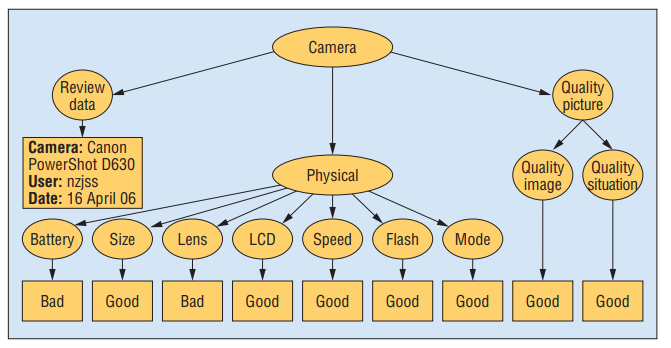
\includegraphics[scale=0.5]{textentailment2.PNG}
      \caption{Taken from \cite{aciar2007informed}}
    \end{figure}
\end{frame}

\begin{frame}{Related work III}
    \begin{itemize}
        \item "Using WordNet-based Context Vectors to Estimate the Semantic Relatedness of Concepts"\\
        \cite{patwardhan2006using}
        \item Uses WordNet definitions to find relatedness between concepts
        \item Can be used to augment queries: For example, "drill" and "saw" might have a high relatedness, if drills are good for a certain recommendation, saws might be too.
        \item Possibly useful in the future when more than one category is added to the system
    \end{itemize}
\end{frame}

\begin{frame}{Related work IV}
    \begin{itemize}
        \item "Recognizing and Justifying Text Entailment through Distributional Navigation on Definition Graphs"\\
        \cite{silva2018recognizing}
        \item The definition graphs can be used to find relevant product categories when the category is not clear: "What is best to make a hole in wood?"
        \item Things that can cut holes would be scissors, drills or saws, but only drills are good here
        \item $\rightarrow$ Find a path between "make\_hole" and product categories containing "wood" in the path
        \item Theorem: \textbf{Product X} has a high score for \textbf{some feature}.
        \item Hypothesis: \textbf{Product X} can be used to cut holes in wood.
    \end{itemize}
\end{frame}

\begin{frame}
\section{Summary}
\frametitle{Summary}
    \begin{itemize}
        \item I will build an ontology containing product specific qualitative knowledge about certain features.
        \item The ontology will be augmented with WordNet definitions to allow question answering in the context of recommending products.
        \item "What is best to make a hole in wood?"
        \item With text entailment and WordNetGraphs from \cite{silva2018recognizing} we can find that drills can do this, but not which drills specifically.
        \item Using my ontology specific products can be identified as being particularly good for certain, specific tasks.
    \end{itemize}
\end{frame}


\begin{frame}[allowframebreaks]{Bibliography}
\bibliographystyle{plainnat}
\bibliography{references}
\end{frame}

\end{document}